\graphicspath{{figtema3/}}

\chapter{Medidas de dispersi\'on}

\section{Introducci\'on}
\label{introTema4}

En el tema anterior hemos visto como los estad\'isticos de
tendencia central resumen en unos pocos valores
el comportamiento global de una distribuci\'on de frecuencias.

Sin embargo, estos estad\'isticos no bastan para describir de manera
suficientemente precisa la distribuci\'on. Consideremos el ejemplo
de la figura \ref{fig1T4}.

\begin{figure}[htbp]
\begin{center}
\begin{tabular}{cc}
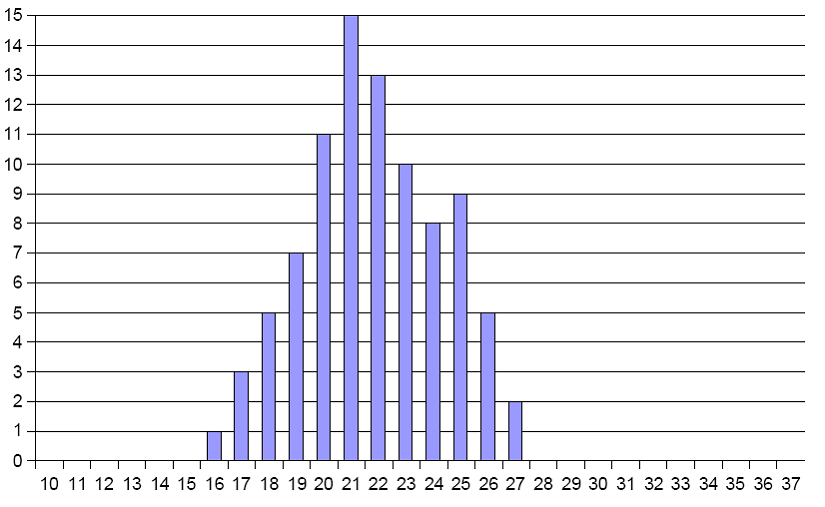
\includegraphics[width=6.5cm]{graf1T4.png} &
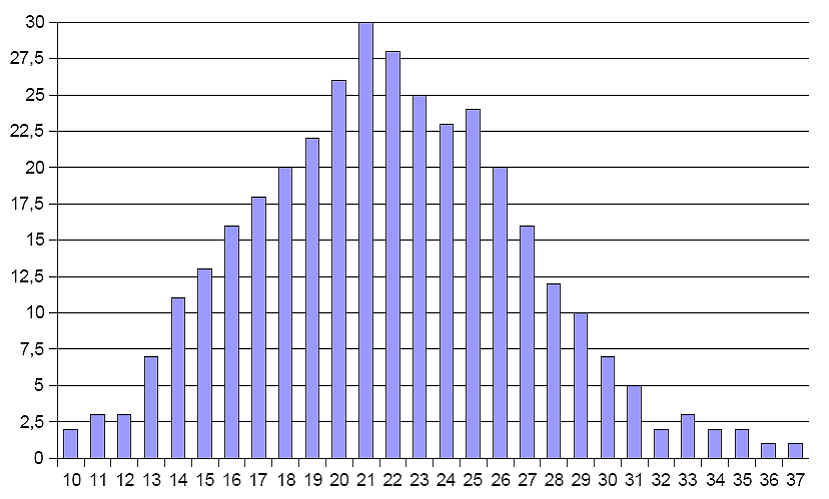
\includegraphics[width=6.5cm]{graf2T4.png} \\
{\small Moda=$21$} & {\small Moda=$21$} \\
{\small Media=$21,82$} & {\small Media=$21,82$} \\
{\small Mediana=$22$} & {\small Mediana=$22$} 
\end{tabular}
\end{center}
\caption{Dos distribuciones diferentes con los mismos estad\'isticos de
tendencia central}
\label{fig1T4}
\end{figure}

Las dos distribuciones de la figura \ref{fig1T4} tienen los mismos valores de
moda, media y mediana. Sin embargo, las distribuciones son bastante diferentes entre s\'i $ $.
En la primera, los valores aparecen concentrados en torno al valor central; en cambio
en la segunda los valores est\'an m\'as dispersos.

En este tema definiremos unos nuevos estad\'isticos cuyos valores dan cuenta de
la heterogeneidad de los datos de la distribuci\'on, por este motivo se llaman
\textbf{medidas de variabilidad} o \textbf{de dispersi\'on}.

\section{Medidas de dispersi\'on}
Las medidas de dispersi\'on m\'as habituales son la varianza y la desviaci\'on t\'ipica.
Sin embargo hay muchas m\'as: rango, rango intercuart\'ilico, 
el \textit{ratio} de variaci\'on, el coeficiente de variaci\'on, etc.
A continuaci\'on definimos cada uno de estos conceptos.

\begin{itemize}
\item \textbf{\textit{Ratio} de variaci\'on}. 
Es una medida de dispersi\'on basada en la moda. Puede utilizarse para cualquier tipo de
variables (cualitativas, ordinales y cuantitativas) con distribuciones unimodales. 
Es la \'unica medida de dispersi\'on que puede calcularse para variables cualitativas.
Se define como:
\[
RV=1-\frac{n_{\text{moda}}}{N}
\]
\noindent
donde $n_{\text{moda}}$ es la m\'axima frecuencia absoluta 
de la distribuci\'on (por tanto la frecuencia de la moda) y $N$ 
es la frecuencia total (la suma de todas las frecuencias absolutas).

Por ejemplo, consideremos la distribuci\'on de la siguiente tabla:

\begin{center}
\begin{tabular}{|c|c|}
\hline
\textit{Nacionalidad} & Frecuencia absoluta \\ \hline
Colombia & 350 \\ \hline
Ecuador & 250 \\ \hline
Per\'u & 120 \\ \hline
Argentina & 100 \\ \hline
Ruman\'ia & 80 \\ \hline
Marruecos & 70 \\ \hline
Senegal & 30 \\ \hline
\end{tabular}
\end{center}

La moda de la variable \textit{Nacionalidad} es \textit{Colombia}, y su frecuencia absoluta
es $350$. La suma de todas las frecuencias absolutas es $1000$, de manera que el ratio de variaci\'on
de la variable es 
\[
RV=1-\frac{350}{1000}=0.65
\]

\textbf{Interpretaci\'on del ratio de variaci\'on}: 
este valor mide el grado de concentraci\'on de los datos en torno a la moda.
Valores cercanos a cero significan que casi todos los valores de la variable est\'an
concentrados en torno al valor de la moda; mientras que valores pr\'oximos a $1$ implican 
que la moda tiene una frecuencia baja y que los valores est\'an dispersos. En resumen:
\[
\text{(concentraci\'on)} \quad 0 \leq VR < 1 \quad \text{(dispersi\'on)}
\]

\item \textbf{Rango}. El rango puede definirse para variables cuantitativas.
Se define como la diferencia entre el valor m\'aximo y el m\'inimo de la variable:
\[
\text{Rango}=\max-\min
\]

A continuaci\'on se muestran los rangos de dos distribuciones de datos diferentes,
correspondientes a ejemplos del tema anterior:

\vskip 0.2 cm
\begin{center}
\begin{tabular}{ll}
\begin{tabular}{|c|c|}
\hline
\textit{Terminaci\'on d\'ecimo ONCE} & Frecuencia\\ \hline
0 & 0 \\ \hline
1 & 4 \\ \hline
2 & 0 \\ \hline
3 & 2 \\ \hline
4 & 2 \\ \hline
5 & 3 \\ \hline
6 & 3 \\ \hline
7 & 6 \\ \hline
8 & 3 \\ \hline
9 & 1 \\ \hline
\end{tabular}
&
\begin{tabular}{l}
Min=$1$ \\
Max=$9$ \\
Rango=$8$
\end{tabular}
\\ \\
%\begin{tabular}{|c|c|}
%\hline
%\textit{Qualificaci\'o} & Frecuencia absoluta \\ \hline
%Suspens & 17 \\ \hline
%Aprovat & 16 \\ \hline
%Notable & 12 \\ \hline
%Excel.lent & 1 \\ \hline
%Matr\'icula d'honor & 3 \\ \hline
%\end{tabular}
%&
%\begin{tabular}{l}
%Min=\textit{Suspens} \\
%Max=\textit{Matr\'icula Honor} \\
%Rango=\textit{Suspens-Matr\'icula Honor}
%\end{tabular}
%\\ \\
\begin{tabular}{|c|c|}
\hline
\textit{Edad} & Frecuencia absoluta \\ \hline
18-19 & 270 \\ \hline
20-21 & 160 \\ \hline
22-23 & 115 \\ \hline
24-25 & 50 \\ \hline
26-27 & 17 \\ \hline
28-29 & 10 \\ \hline
30-40 & 4 \\ \hline
\end{tabular} 
&
\begin{tabular}{l}
Min=$18$ \\
Max=$40$ \\
Rango=$22$
\end{tabular}

\end{tabular}

\end{center}

\noindent
Remarcar que para la primera tabla el valor m\'inimo en la muestra no es cero pues su frecuencia es cero.
El valor m\'inimo es el primer valor cuya frecuencia es distinta de cero.
En cuanto a la segunda tabla, hemos tomado como valores m\'aximo
y m\'inimo el l\'imite inferior del primer intervalo y el superior del \'ultimo.
Otra opci\'on igualmente v\'alida hubiera sido tomar los valores medios de
estos intervalos.


\vskip 0.3 cm
\textbf{Interpretaci\'on del rango}: en general podemos afirmar que
para valores similares de media, moda o mediana, valores grandes 
del rango implican 
mayor dispersi\'on que valores m\'as peque\~nos. 
Sin embargo esto no siempre es cierto,
como veremos a continuaci\'on.


\item \textbf{Rango intercuart\'ilico (RIC)}.
Para entender el significado de este estad\'istico consideremos primero los siguientes 
ejemplos:

\vskip 0.2 cm
\begin{center}
\begin{tabular}{cc}
\begin{tabular}{|c|c|}
\hline
\textit{Edad} & Frecuencia \\ \hline
18 & 5 \\ \hline
19 & 17 \\ \hline
20 & 12 \\ \hline
21 & 9 \\ \hline
22 & 9 \\ \hline
23 & 8 \\ \hline
24 & 4 \\ \hline
\end{tabular} 
&
\begin{tabular}{|c|c|}
\hline
\textit{Edad} & Frecuencia \\ \hline
18 & 5 \\ \hline
19 & 17 \\ \hline
20 & 12 \\ \hline
21 & 9 \\ \hline
22 & 9 \\ \hline
23 & 8 \\ \hline
24 & 4 \\ \hline
35 & 1 \\ \hline
\end{tabular} 
\\
Moda=19 & Moda=19 \\
Mediana=19 & Mediana=19 \\
Media=20,62 & Media=20,84 \\
Min=18 & Min=18 \\
Max=24 & Max=35  \\
Rango=6 & Rango=17
\end{tabular}
\end{center}

\noindent
Observamos como en la segunda tabla, un solo valor extremo ($35$, con frecuencia $1$)
provoca que el rango de ambas distribuciones sea muy distinto, cuando en realidad
ambas contienen pr\'acticamente los mismos valores.

Este ejemplo muestra que el rango es muy sensible a los valores extremos de la distribuci\'on.
Una medida de dispersi\'on m\'as robusta es el rango intercuart\'ilico, que se define
como la diferencia entre el tercer cuartil y el primer cuartil:
\[
\text{RIC}=3^{er} \text{cuartil} - 1^{er} \text{cuartil}
\]

Para las tablas anteriores tendr\'iamos: $1^{er}$ cuartil=$19$ (para ambas tablas),
$3^{\mathrm{er}}$ cuartil=$22$ (para ambas tablas). De manera que en ambos casos tenemos RIC=$22-19=3$.


\vskip 0.3 cm
\textbf{Interpretaci\'on del rango intercuart\'ilico}. La interpretaci\'on es la misma que
la del rango: un valor grande implica mayor dispersi\'on que uno peque\~no. Sin embargo, 
el rango intercuart\'ilico presenta la ventaja de ser robusto ante valores extremos poco frecuentes,
por eso se utiliza m\'as que el rango. Adem�s, el $50\%$ de los valores centrales de la 
muestra se encuentran entre los l�mites del RIC.

%Por otra parte, el RIC es tambi\'en el tama\~no del intervalo central de la distribuci\'on que contiene
%el $50\%$ de los valores de la variable (ver figura \ref{ilustrRIC}). 
%
%\begin{figure}
%\begin{center}
%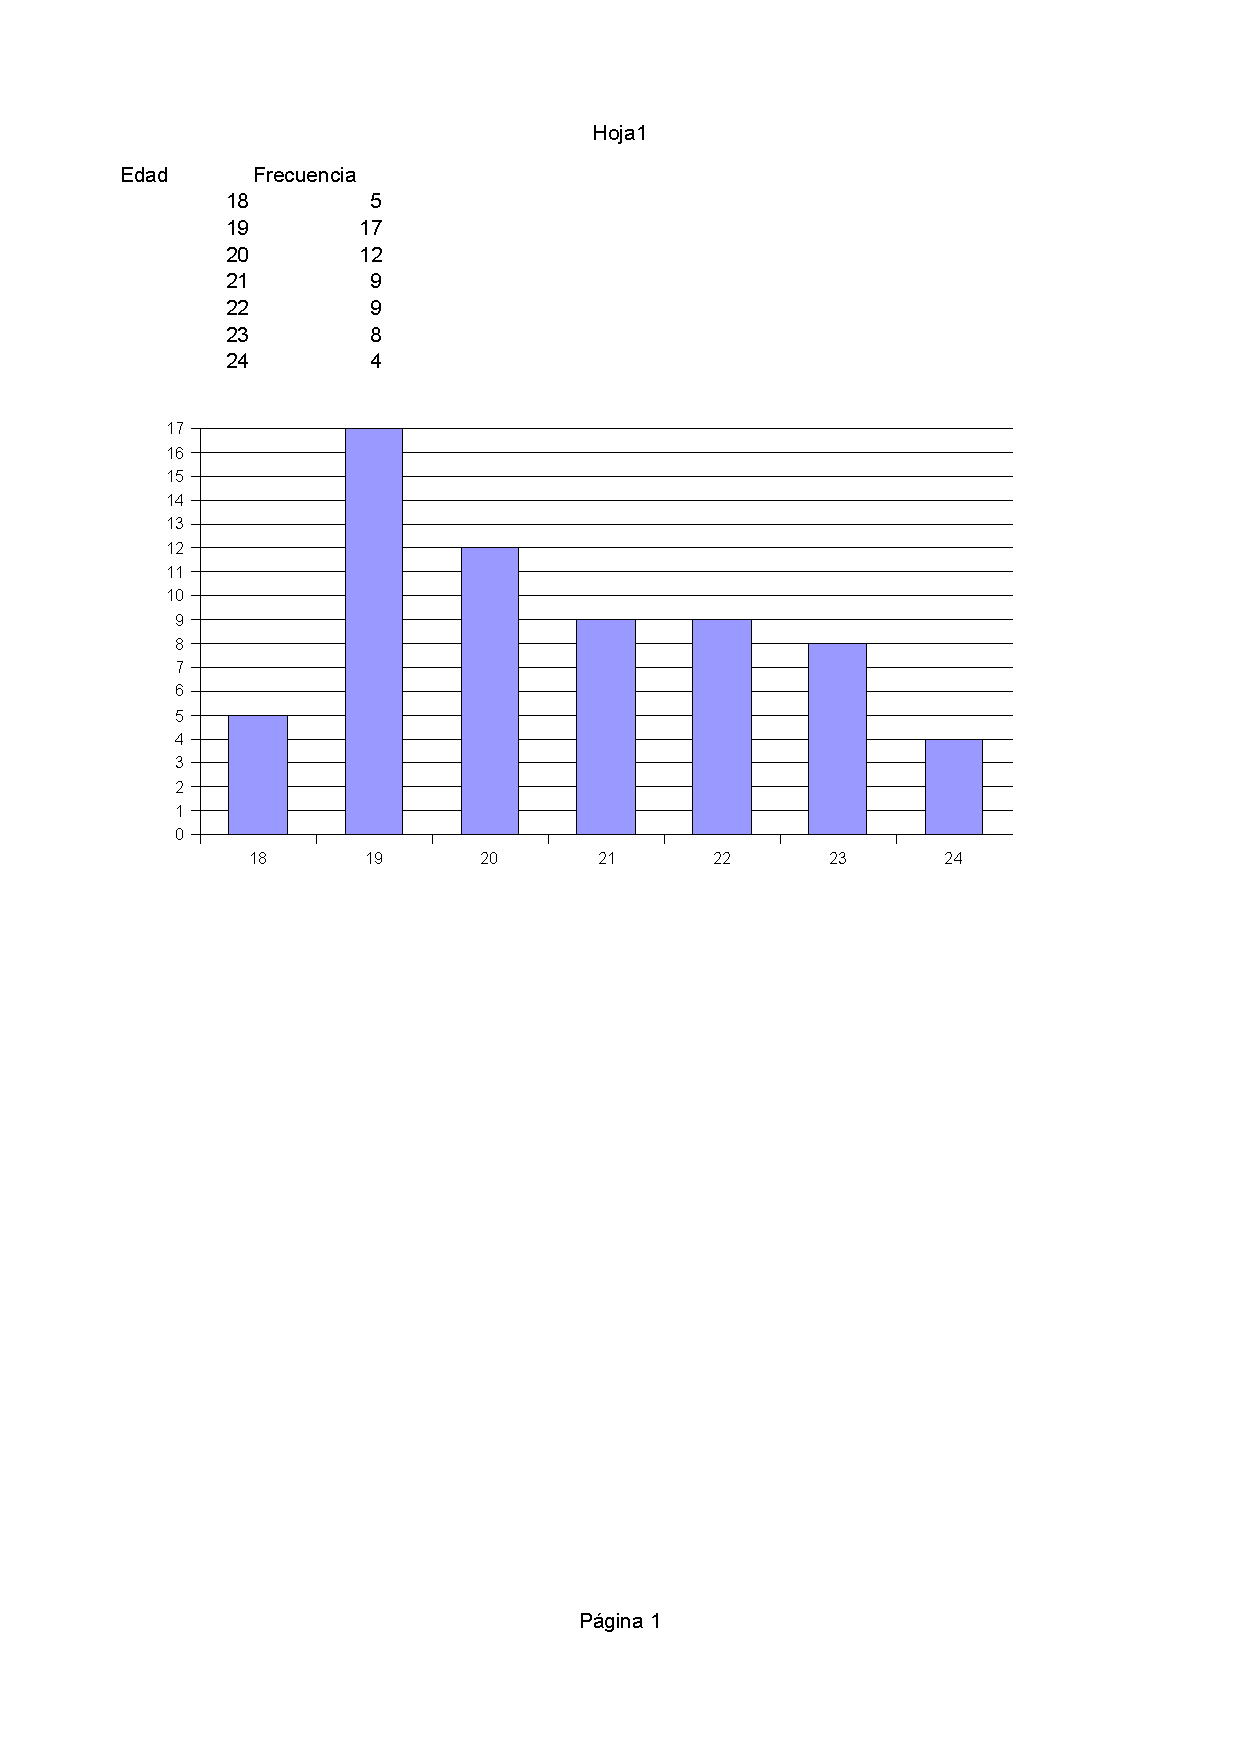
\includegraphics[width=8cm]{ilustrRIC.png}
%\end{center}
%\caption{El RIC es el tama\~no del intervalo central de la distribuci\'on 
%que contiene el $50\%$ de los valores de la variable}
%\label{ilustrRIC}
%\end{figure}

\item \textbf{Varianza}. La varianza es una medida de dispersi\'on que s\'olo 
puede utilizarse para variables cuantitativas. Su definici\'on depende de si
se aplica a datos de una poblaci\'on o una muestra:
\[
\begin{array}{l}
\text{Var}=\frac{\sum_{i=1}^k n_i \cdot (x_i-\bar{x})^2}{N}=
\frac{n_1 \cdot (x_1-\bar{x})^2+n_2 \cdot (x_2-\bar{x})^2+\cdots+n_k(x_k-\bar{x})^2}{N} \\
 \text{(varianza poblacional)} \\ \\
\text{Var}=\frac{\sum_{i=1}^k n_i \cdot (x_i-\bar{x})^2}{N-1}=
\frac{n_1 \cdot (x_1-\bar{x})^2+n_2 \cdot (x_2-\bar{x})^2+\cdots+n_k(x_k-\bar{x})^2}{N-1} \\
 \text{(varianza muestral)}
\end{array}
\]
\noindent
donde $x_i$ representa los distintos valores de la variable, $n_i$ sus frecuencias,
$k$ es el n\'umero de valores diferentes que toma la variable, $N=n_1+n_2+ \cdots+n_k$ 
y $\bar{x}$ es la media de los valores.

Como ya vimos en el tema 1, el t\'ermino \textit{poblaci\'on} hace referencia al total
de individuos sobre los que se evalua una variable estad\'istica, mientras que
una \textit{muestra} es una peque\~na porci\'on de la poblaci\'on total.
Cuando la varianza se calcula sobre el total de datos posibles de una variable
empleamos la f\'ormula de la varianza poblacional. Cuando los datos disponibles representan
una peque\~na porci\'on del total de datos posibles empleamos la f\'ormula de la varianza muestral. 
El por qu\'e de esta distinci\'on entre ambos tipos de varianza se explicar\'a en el m�dulo III.


\vskip 0.3 cm
Tomemos por ejemplo los datos de la siguiente tabla, ya utilizada en el tema anterior
(ver ejemplo 2, secci\'on \ref{secCentralOrd}):
\vskip 0.2 cm
%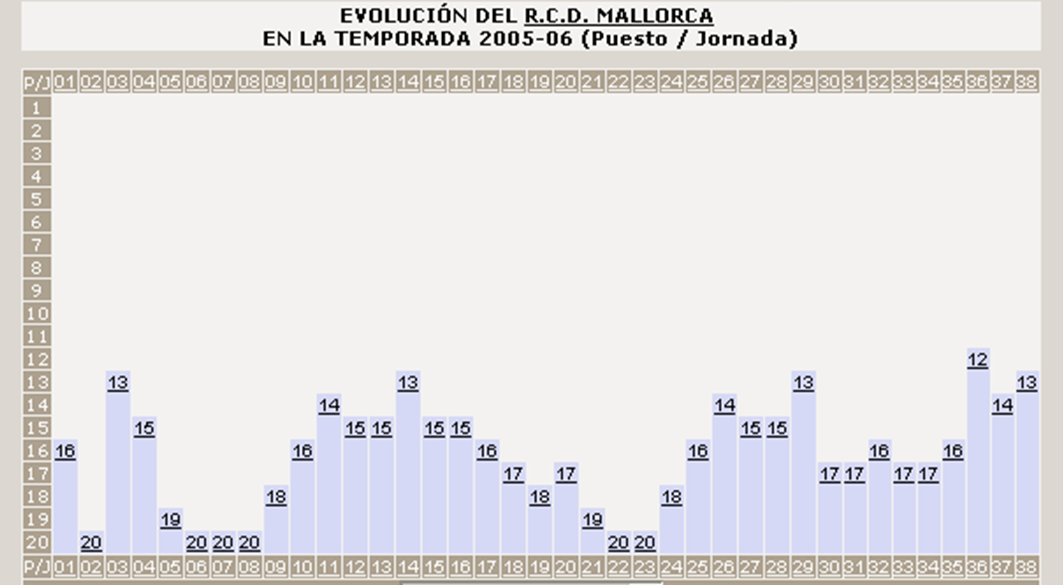
\includegraphics[width=14cm]{ejemplo5T2.png}
\begin{center}
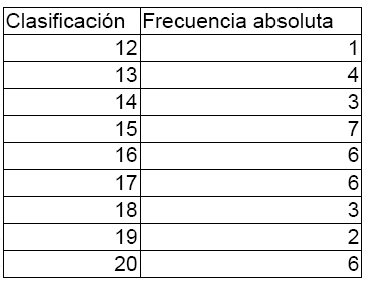
\includegraphics[width=6cm]{ejemplo1.png}
\end{center}

El objeto del estudio es analizar la clasificaci\'on de un equipo de f\'utbol (RCD Mallorca)
durante la temporada 2005-2006. Los datos de la tabla muestran \emph{todos} los valores de
la clasificaci\'on durante ese a\~no, por lo que podemos considerar que son datos
poblacionales. De manera que utilizaremos la primera versi\'on de la f\'ormula de la 
varianza:
\[
\begin{array}{ll}
\text{Var}&=\frac{1 \cdot (12-16,34)^2+ 4 \cdot (13-16,34)^2+ \cdots+
6 \cdot (20-16,34)^2}{1+4+\cdots +6}= \\ \\ 
&=5,23
\end{array}
\]
\noindent
donde se ha utilizado que $\bar{x}=16,34$, que es el valor de la media obtenido en el tema 
anterior.

\vskip 0.3 cm
Como segundo ejemplo consideremos los datos de la tabla \ref{tabedadUIB}.

\begin{table}
\begin{center}
\caption{Edad estudiantes UIB}
\label{tabedadUIB}
\vskip 0.2 cm
\begin{tabular}{|c|c|}
\hline
\textit{Edad} & Frecuencia absoluta \\ \hline
18 & 120 \\ \hline
19 & 150 \\ \hline
20 & 90 \\ \hline
21 & 70 \\ \hline
22 & 65 \\ \hline
23 & 50 \\ \hline
24 & 30 \\ \hline
25 & 20 \\ \hline
26 & 10 \\ \hline
27 & 7 \\ \hline
28 & 8 \\ \hline
29 & 2 \\ \hline
30 & 1 \\ \hline
34 & 1 \\ \hline
35 & 1 \\ \hline
40 & 1 \\ \hline
\end{tabular}
\end{center}
\end{table}

Estos datos corresponden a un estudio sobre la edad de los estudiantes de la UIB,
pero en lugar de tener datos de \textbf{todos} los estudiantes de la UIB s\'olo disponemos
de datos de 626 estudiantes. Debemos calcular por tanto la varianza muestral:
\[
\begin{array}{ll}
\text{Var}&=\frac{120 \cdot (18-20,69)^2+ 150 \cdot (19-20,69)^2+ \cdots+
40 \cdot (40-20.69)^2}{(120+150+\cdots +1)-1}=\\ \\
&= 7,03
\end{array}
\]
\noindent
donde se ha utilizado que $\bar{x}=20,69$, que es el valor de la media obtenido en el tema 
anterior.


\vskip 0.5 cm
\noindent
\textbf{C\'alculo de la varianza para variables descritas por intervalos}

El procedimiento es muy similar al utilizado para la media en el tema anterior 
(secci\'on \ref{secintervals}).
Calculamos en primer lugar los puntos medios de los intervalos. 
Si los limites de un intervalo son $L_i$ y $L_{i+1}$, el punto medio es 
$m_i=\displaystyle \frac{L_i + L_{i+1}}{2}$.

Para el ejemplo de los estudiantes de la UIB:

\vskip 0.2 cm
\begin{center}
\begin{tabular}{|c|c|c|}
\hline
\textit{Edad} (intervalo) & \textit{Edad} (punto medio) &Frecuencia absoluta \\ \hline
18-19 & 18,5 & 270 \\ \hline
20-21 & 20,5 & 160 \\ \hline
22-23 & 22,5 & 115 \\ \hline
24-25 & 24,5 & 50 \\ \hline
26-27 & 26,5 & 17 \\ \hline
28-29 & 28,5 & 10 \\ \hline
30-40 & 35 & 4 \\ \hline
\end{tabular}
\end{center}

La varianza se calcula con una f\'ormula muy parecida a la de la secci\'on anterior:
\[
\begin{array}{l}
\text{Var}=\frac{\sum_{i=1}^k n_i \cdot (m_i-\bar{x})^2}{N}=
\frac{n_1 \cdot (m_1-\bar{x})^2+n_2 \cdot (m_2-\bar{x})^2+\cdots+n_k(m_k-\bar{x})^2}{N} \\ 
  \text{(varianza poblacional)} \\ \\
\text{Var}=\frac{\sum_{i=1}^k n_i \cdot (m_i-\bar{x})^2}{N-1}=
\frac{n_1 \cdot (m_1-\bar{x})^2+n_2 \cdot (m_2-\bar{x})^2+\cdots+n_k(m_k-\bar{x})^2}{N-1} \\
  \text{(varianza muestral)}
\end{array}
\]
\noindent
donde $k$ es el n\'umero total de intervalos, $m_i$ el punto medio del intervalo $i$,
$n_i$ su frecuencia , $N$ la suma de todas las frecuencias y $\bar{x}$ la media.

En nuestro caso calculamos la varianza muestral, por las mismas razones que en el ejemplo
anterior:
\[
\begin{array}{ll}
\text{Var}&=\frac{270 \cdot (18,5-20,7)^2+ 160 \cdot (20,5-20,7)^2+ \cdots+
4 \cdot (35-20,7)^2}{(270+160+\cdots +4)-1}= \\ \\
&=7,05
\end{array}
\]
\noindent
donde se ha utilizado que $\bar{x}=20,7$, que es el valor de la media obtenido en el tema 
anterior.

\vskip 0.5 cm
\noindent
\textbf{C\'alculo de la varianza a partir de datos brutos}
Al igual que ocurr�a con el c�lculo de la media, el c�lculo de la varianza a partir 
de datos brutos puede hacerse de una manera muy sencilla utilizando las siguientes
f�rmulas:

\[
\begin{array}{ll}
\mathrm{Var}=\frac{\sum_{i=1}^N x_i^2}{N} - \bar{x}^2=
\frac{x_1^2+x_2^2+\cdots+x_N^2}{N} - \bar{x}^2
& \text{(varianza poblacional)} \\ \\
\mathrm{Var}=\frac{\sum_{i=1}^N x_i^2}{N-1} - \frac{N}{N-1}\bar{x}^2=
\frac{x_1^2+x_2^2+\cdots+x_N^2}{N-1} - \frac{N}{N-1}\bar{x}^2
& \text{(varianza muestral)} 
\end{array}
\]

\noindent
donde $x_i$ representa los distintos valores de la variable, $N$ es el n�mero total
de valores y $\bar{x}$ su media.

\vskip 0.3 cm
Consideremos por ejemplo los datos de la siguiente tabla, en la que se muestran las
notas de varios alumnos de la asignatura de Econom�a:

\vskip 0.2 cm
\begin{center}
\begin{tabular}{c|c}
 & Nota \\
\hline
 Alumno 1 & 7 \\
 Alumno 2 & 6,5 \\
 Alumno 3 & 8 \\
 Alumno 4 & 4,5 \\
 Alumno 5 & 9 \\
 Alumno 6 & 3,5 \\
 Alumno 7 & 8 \\
 Alumno 8 & 7 \\
 Alumno 9 & 4,5 \\
 Alumno 10 & 5
\end{tabular}
\end{center}

Queremos analizar las notas de estos 10 alumnos pero no deseamos 
extrapolar nuestros resultados al an�lisis de un grupo mayor, por lo
que calcularemos la varianza poblacional.

\vskip 0.2 cm
En el tema anterior se ha calculado la media de estos datos ($\bar{x}=6,3$).
La varianza se calcula de la siguiente forma:
\[
\begin{array}{ll}
\mathrm{Var}&=\frac{7^2+6,5^2+8^2+4,5^2+9^2+3,5^2+8^2+7^2+4,5^2+5^2}{10}-6,3^2= \\ \\
&=3,01
\end{array}
\]


\vskip 0.5 cm
\textbf{Interpretaci\'on de la varianza}: la varianza mide la dispersi\'on media 
de los valores de la variable. Valores grandes 
de la varianza significan gran dispersi\'on respecto al valor medio mientras
que valores peque\~nos implican una dispersi\'on menor.


\item \textbf{Desviaci\'on t\'ipica}. Tambi\'en llamada \textbf{desviaci\'on est\'andar},
se calcula simplemente como la ra\'iz cuadrada de la varianza (sea�\'esta poblacional o muestral):
\[
\text{desviaci\'on est\'andar}=s=\sqrt{\text{Var}}
\]

Al igual que la varianza la desviaci\'on t\'ipica s\'olo puede calcularse para
variables cuantitativas.
Para los ejemplos de la secci\'on anterior:
\vskip 0.2 cm
\begin{center}
\begin{tabular}{ll}
Clasificaci\'on RCD Mallorca 2005-2006: & $\sqrt{5,23}=2.29$ \\ \\
Edad estudiantes UIB (sin agrupar en intervalos): & $\sqrt{7,03}=2,651$\\ \\
Edad estudiantes UIB (agrupando en intervalos): & $\sqrt{7,05}=2,655$
\end{tabular}
\end{center}

\vskip 0.5 cm
\textbf{Interpretaci\'on de la desviaci\'on est\'andar}: al igual que la varianza
la desviaci\'on t\'ipica mide la dispersi\'on media 
de los valores de la va\-ria\-ble. Cuanto mayor sea el valor mayor ser\'a la dispersi\'on
respecto al valor medio.

Una propiedad \'util que relaciona los valores de media y desviaci\'on t\'ipica 
con la manera en que se distribuyen los datos de la variable es la 
\textbf{desigualdad de Chebychev}. Seg\'un esta desigualdad, la proporci\'on de
valores de la variable en el intervalo 
$[\bar{x}-k \cdot s, \bar{x}+k \cdot s]$ es, como m\'inimo,  
$\displaystyle (1-\frac{1}{k^2}) \times 100\% $, donde $\bar{x}$ y $s$ son, respectivamente,
la media y la desviaci\'on t\'ipica de la variable.

Aplicando esta propiedad a distintos valores de $k$ tenemos, por ejemplo:

\begin{itemize}
\item al menos el $75\%$ de los datos est\'an entre $[\bar{x}-2 \cdot s$ y  $\bar{x}+2 \cdot s]$
\item al menos el $89\%$ de los datos est\'an entre $[\bar{x}-3 \cdot s$ y  $\bar{x}+3 \cdot s]$
\item al menos el $93.75\%$ de los datos est\'an entre $[\bar{x}-4 \cdot s$ y  $\bar{x}+4 \cdot s]$
\end{itemize}

\vskip 0.3 cm
Por ejemplo, para los datos sobre la edad de los estudiantes de la UIB (sin agrupaci\'on en intervalos)
ten\'iamos $\bar{x}=20,69$ y $s=2,65$. De acuerdo con la propiedad anterior deber\'ia cumplirse que
al menos el $75\%$ de los datos est\'a entre $20,69-2 \cdot 2,65=15,39$ y 
$20,69+2 \cdot 2,65=25,99$. Los valores de la variable \textit{Edad} en este intervalo son: 
$18$, $19$, $20$, $21$, $22$, $23$, $24$ y $25$. Y la suma de las frecuencias de estos valores
es: $120+150+90+70+65+50+30+20=595$. Esta cantidad representa un 
$\frac{595}{626} \times 100\%=95\%$ del total de datos, por lo que, en efecto, se cumple la propiedad.

\item \textbf{Coeficiente de variaci\'on}. Es el cociente entre la desviaci\'on est\'andar y la
media de una variable. S\'olo se define para variables cuantitativas positivas.
\[
CV=\frac{s}{\bar{x}}
\]


\vskip 0.5 cm
\noindent
\textbf{Interpretaci\'on del coeficiente de variaci\'on}. Este coeficiente nos dice 
c�antas medias caben en $s$.
Normalmente las variables cuyo valor medio es mayor presentan una varianza
tambi\'en mayor. Por ello, no tiene mucho sentido comparar las varianzas (o desviaciones
t\'ipicas) de dos variables con valores de media muy diferentes. En estos casos
es mejor comparar sus coeficientes de variaci\'on. Un mayor valor del coeficiente
implica una mayor dispersi\'on de los datos.

\vskip 0.3 cm
Para los ejemplos de las secciones anteriores:
\vskip 0.2 cm
\begin{center}
\begin{tabular}{ll}
Clasificaci\'on RCD Mallorca 2005-2006: & $CV=\frac{2,29}{16,34}=0,14$ \\ \\
Edad estudiantes UIB (sin agrupar en intervalos): & $CV=\frac{2,65}{20,69}=0,128$
\end{tabular}
\end{center}


\end{itemize}


\section{Tipificaci�n de variables estad�sticas (\textit{z-scores})}

En ocasiones debemos comparar valores de una misma variable obtenidos
a partir de distintos datos estad�sticos. Un ejemplo t�pico es el siguiente:

\vskip 0.3 cm
Una asignatura se imparte en dos grupos distintos por diferentes profesores,
cada profesor pone un examen diferente, m�s dif�cil en el grupo 1 que en el grupo 2.
Al estudiante con mejor nota se le concede una matr�cula gratuita para el curso siguiente.
El mejor alumno del primer grupo tiene una nota de $8$, mientras que el del segundo grupo
de $9$. ?`Es justo concederle la matr�cula gratuita al alumno del segundo grupo sabiendo que
su examen ha sido m�s f�cil? Si conocemos la media y la desviaci�n t�pica (o varianza) 
de las notas de ambos grupos es posible decidir qu� alumno es realmente mejor con ayuda 
de la tipificaci�n.

\vskip 0.3 cm
La \textit{tipificaci�n} normaliza o estandariza los valores de las variables obtenidos a partir
de conjuntos de datos diferentes. El valor tipificado (tambi�n llamado \textit{z-score})
se calcula del siguiente modo:
\[
z=\frac{|v-\bar{x}|}{s}
\]
\noindent
donde $\bar{x}$ y $s$ son, respectivamente, la media y la varianza del conjunto de datos
al que pertenece el valor $v$. El s\'imbolo $| \qquad |$ denota el valor absoluto y significa 
que el valor de $v-\bar{x}$ se toma siempre con signo positivo.

Los datos tipificados pueden ya compararse de manera directa.
Para nues\-tro ejemplo, si las notas medias de ambos grupos son $\bar{x}_1=6$ y  
$\bar{x}_2=7$, y las desviaciones t�picas $s_1=1,5$ y $s_2=2$, respectivamente, los 
\textit{z-scores} de los mejores alumnos ser�n:
\[
z_1=\frac{8-6}{1,5}=1,33 \qquad \qquad z_2=\frac{9-7}{2}=1
\]

\noindent
como $z_1 > z_2$ probablemente el mejor alumno es el del primer grupo, aunque su nota sea inferior.



\section{Diagramas de caja}

Los diagramas de caja son representaciones gr\'aficas que permiten vi\-sua\-lizar de
manera r\'apida la dispersi\'on de los valores de una variable.
En estos diagramas se muestran la mediana, el rango intercuart\'ilico, los
valores ``at\'ipicos'' y los valores ``extremos''.

La figura \ref{diagcaja1} muestra de forma esquem\'atica un diagrama de caja 
y los valores que lo definen. Calcularemos por ejemplo el diagrama de caja
co\-rres\-pon\-dien\-te a la tabla \ref{tabedadUIB}.

\begin{figure}[htbp]
\begin{center}
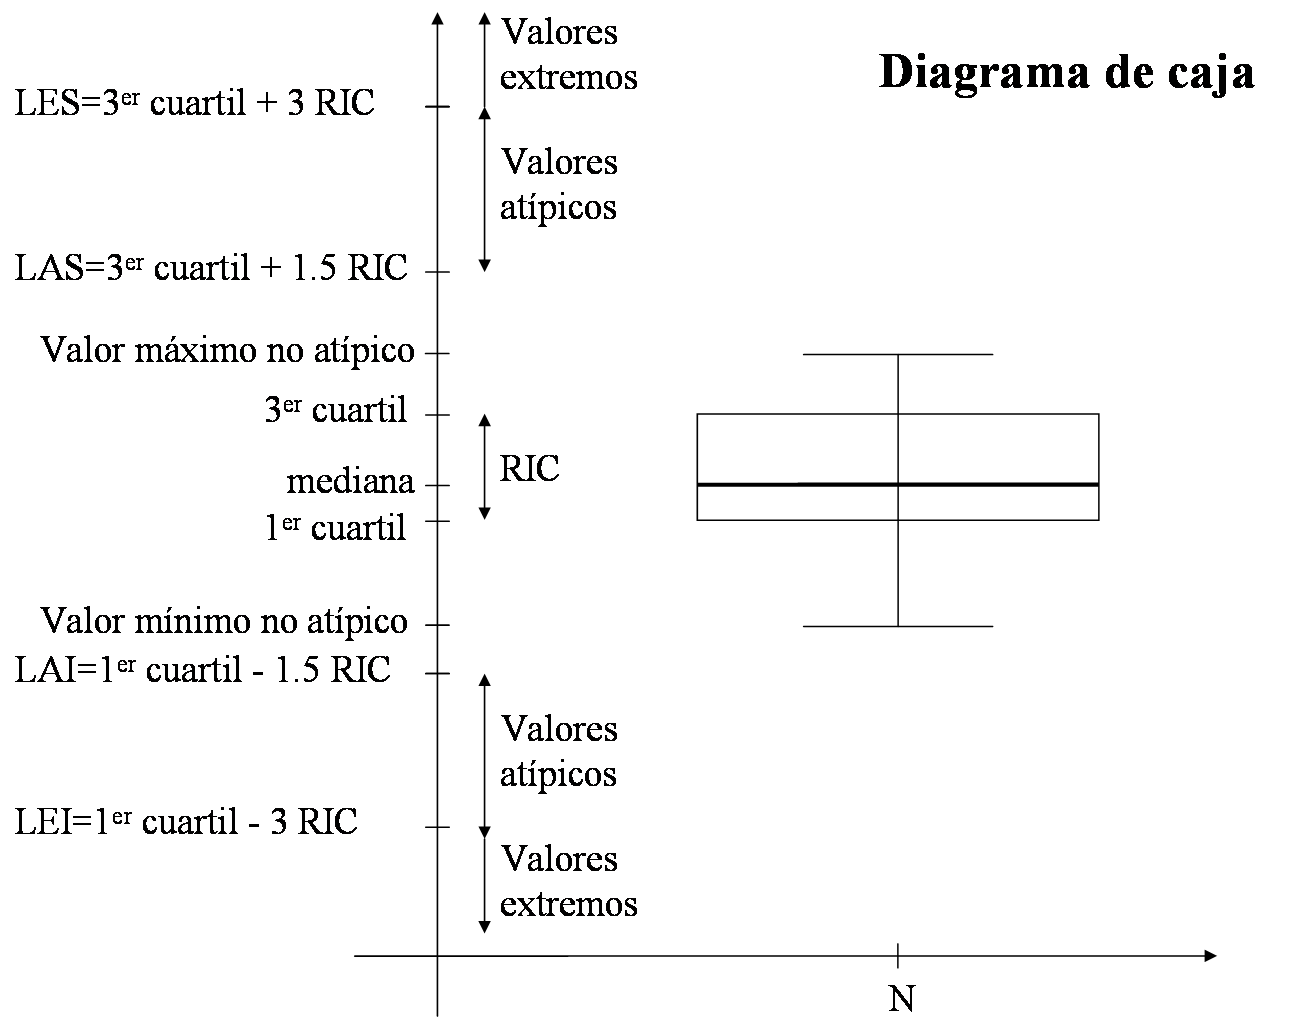
\includegraphics[width=14cm]{diagcaja1.png}
\end{center}
\caption{Representaci\'on esquem\'atica de un diagrama de caja}
\label{diagcaja1}
\end{figure}

El diagrama de caja presenta las siguientes caracter\'isticas:
\begin{itemize}
\item El eje vertical representa los valores de la variable. 
En el eje horizontal se indica la frecuencia acumulada total y el diagrama es sim\'etrico
respecto a este valor.
\item El rango intercuat\'ilico se representa mediante un rect\'angulo.
El borde inferior del rect\'angulo representa el primer cuartil y el superior
el tercer cuartil. La altura del rect\'angulo es por tanto igual al rango intercuart\'ilico (RIC).
La anchura del rect\'angulo no tiene ning\'un significado.

Dentro del rect\'angulo una l\'inea m\'as gruesa indica
el valor de la me\-dia\-na. 
Al menos el $50\%$ de los valores de la variable se encuentran dentro de este 
rect\'angulo.

En nuestro ejemplo los l\'imites del rect\'angulo son: $1^{er}$ cuartil=$19$ y
$3^{er}$ cuartil=$22$ (ver figura \ref{diagcaja2}).

\item Para definir los valores ``at\'ipicos'' y ``extremos'' se utilizan
los siguientes l\'imites (aunque en algunos autores utilizan otros):

\[
\begin{array}{l}
\text{l\'imite at\'ipico inferior (LAI)} =1^{er} \text{cuartil} - 1,5 \times RIC \\ \\
\text{l\'imite at\'ipico superior (LAS)}=3^{er} \text{cuartil} + 1,5 \times RIC \\ \\
\text{l\'imite extremo inferior (LEI)}=1^{er} \text{cuartil} - 3 \times RIC \\ \\
\text{l\'imite extremo superior (LES)}=3^{er} \text{cuartil} + 3 \times RIC 
\end{array}
\]

Se denominan \textbf{valores at\'ipicos} aquellos valores que se encuentran
entre LAI y LEI o bien entre LAS y LES. Son \textbf{valores extremos}
aquellos inferiores a LEI o superiores a LES (ver figura \ref{diagcaja1}).

En nuestro ejemplo $RIC=3$, por lo que estos l\'imites son:
\[
\begin{array}{l}
\text{LAI}=19 - 1,5 \cdot 3 = 14,5\\ \\
\text{LAS}=22 + 1,5 \cdot 3 = 26,5 \\ \\
\text{LEI}=19 - 3 \cdot 3 = 10\\ \\
\text{LES}=22 + 3 \cdot 3 = 31 \\ \\
\end{array}
\]

En el diagrama de caja se marcan con $\circ$ los valores at\'ipicos y con $\bullet$ los extremos.
En nuestro ejemplo (ver figura \ref{diagcaja2}) son valores at\'ipicos aquellos que est\'an entre 
$10$ y $14,5$ (no incluido) y entre $26,5$ (no incluido) y $31$: $27$, $28$, $29$, $30$. 
Son valores extremos los inferiores a $10$ y los superiores a $31$: $34$, $35$, $40$.


\item Por \'ultimo, en el diagrama se marcan con dos l\'ineas horizontales los valores m\'aximo y 
m\'inimo no at\'ipicos (ver figura \ref{diagcaja1}). En nuestro ejemplo el m\'aximo valor
no at\'ipico de la variable es $26$ (inferior a LAS); mientras que el m\'inimo valor
no at\'ipico es $18$ (superior a LAI). Estos dos valores se conectan con el rect\'angulo mediante l\'ineas
verticales (ver figura \ref{diagcaja1} y \ref{diagcaja2}). 

\end{itemize}


En la figura \ref{diagcaja2} se muestra el diagrama de caja correspondiente
a los datos de la tabla \ref{tabedadUIB}.

\begin{figure}[htbp]
\begin{center}
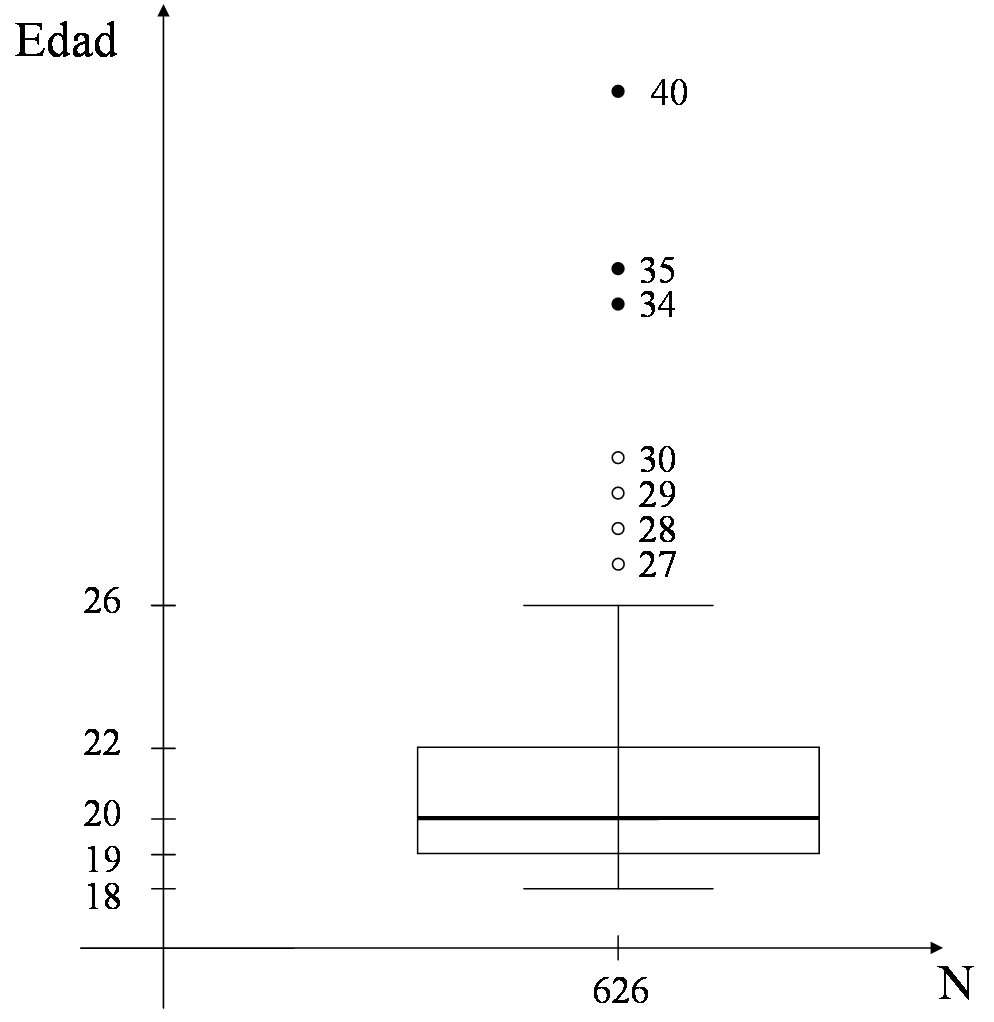
\includegraphics[width=12cm]{diagcaja2.png}
\end{center}
\caption{Diagrama de caja correspondiente a los datos de la tabla \ref{tabedadUIB}}
\label{diagcaja2}
\end{figure}


\section{C\'alculo de medidas de dispersi\'on con el ordenador}
Las operaciones matem\'aticas que deben realizarse para calcular los estad\'isticos
explicados en este tema son muy sencillas y pueden realizarse con una simple calculadora.
No obstante, si la cantidad de datos es elevada, programas como la hoja de c�lculo
 OpenOffice Calc permiten 
c\'alcular f\'acilmente los estad\'isticos m\'as habituales de una distribuci\'on. 
Explicaremos c\'omo ha\-cer\-lo en los siguientes ejemplos.


\vskip 0.5 cm
\noindent
\textbf{Ejemplo 1}

Calcular el \textit{ratio} de variaci\'on de la variable ``tipo de
infracci\'on'' a partir de los datos de la siguiente tabla:

\begin{center}
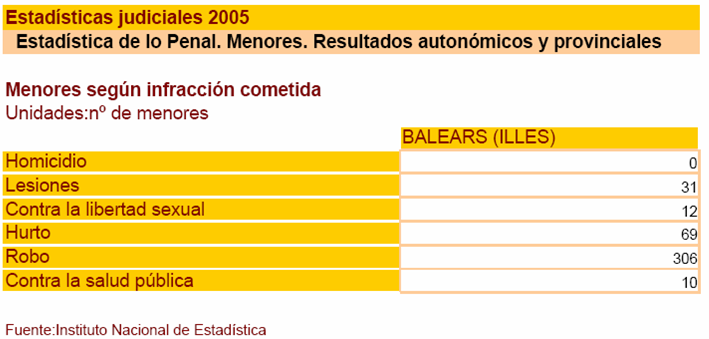
\includegraphics[width=13cm]{ejemplo4.png}
\end{center}

\vskip 0.3 cm
El c\'alculo es sencillo y puede hacerse con la ayuda de una calculadora.
El modo de la variable es \textit{Robo}, cuya frecuencia es $306$.
La suma de todas las frecuencias es $N=31+12+69+306+10=428$. De manera que:
\[
RV=1-\frac{306}{428}=0,28=28\%
\]

Este valor indica que s\'olo el $28\%$ de los valores de la variable se
encuentran fuera de la categor\'ia \textit{Robo}, o lo que es lo mismo,
la mayor\'ia de valores se concentran en la moda.

\vskip 0.5 cm
\noindent
\textbf{Ejemplo 2}

Calcular el rango, rango intercuart\'ilico, varianza, desviaci\'on est\'andar,
valores at\'ipicos y valores extremos para la variable 
``autobuses matriculados por mes durante el a\~no 2006'' 
a partir de los datos de la siguiente tabla (fuente DGT):

\begin{center}
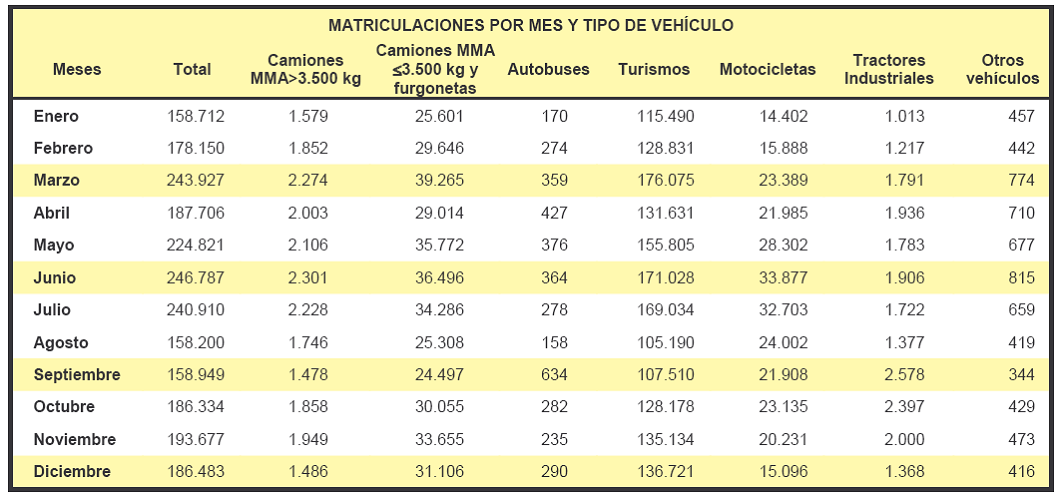
\includegraphics[width=13.5cm]{ejemplo5.png}
\end{center}

\vskip 0.3 cm
Los datos de esta tabla ya se han utilizado en el tema anterior.
Se trata de datos en bruto que deben escribirse en un documento de
OpenOffice Calc, tal como muestra la figura \ref{calc1ej5T2b}

\begin{figure}[htbp]
\begin{center}
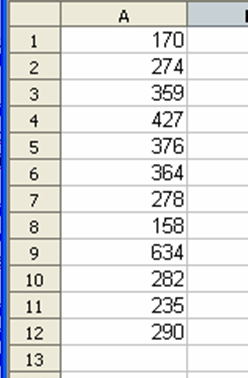
\includegraphics[width=3cm]{calc1ej5T2.png}
\end{center}
\caption{Datos \textit{brutos} del ejemplo 2}
\label{calc1ej5T2b}
\end{figure}

El procedimiento para el c\'alculo de la mediana y los cuartiles se ha explicado
en el ejemplo 6 del tema anterior. Recordemos los resultados: 
mediana=$286$, $1^{er}$ cuartil=$264,25$ y $3^{er}$ cuartil =$367$.
El rango intercuart\'ilico es por tanto: $RIC=367-264,25=102,75$.

El c\'alculo de la varianza, la desviaci\'on t\'ipica y el rango es muy sencillo
con Calc cuando se dispone de valores brutos. Para este ejemplo:
\begin{enumerate}
\item Escribimos las palabras ``Varianza'', ``Desv. t�pica'', ``M\'inimo'',
``M\'aximo'' y ``Rango'' en
las casillas $C20$ a $C24$, por ejemplo, de la hoja de c\'alculo.
\item \textbf{Varianza}. Debemos decidir primero si consideramos que los datos
se refieren a una \textit{poblaci\'on} o a una \textit{muestra}.
Dado que la variable bajo estudio es 
``autobuses matriculados por mes durante el a\~no 2006'' y disponemos de \emph{todos}
los datos de este a\~no, podemos considerar que se trata de datos de poblaci\'on.

Para el c\'alculo
nos situamos en la casilla $D20$ y escribimos \verb@=Varp(A1:A12)@. Al pulsar 
\textit{Enter} obtenemos el valor de la varianza poblacional. (Si hubi\'eramos querido calcular 
la varianza muestral la f\'ormula hubiera sido \verb@=Vara(A1:A12)@).

\item \textbf{Desviaci\'on est\'andar}.
Nos situamos en la casilla $D21$ y escribimos \verb@=Ra�z(D20)@. Al pulsar 
\textit{Enter} obtenemos el valor de la desviaci\'on est\'andar. 

\item \textbf{M\'inimo}. Nos situamos en la casilla $D22$ y escribimos \verb@=M�n(A1:A12)@. 
Al pulsar  \textit{Enter} obtenemos el valor de m\'inimo de la variable.

\item \textbf{M\'aximo}. Nos situamos en la casilla $D23$ y escribimos \verb@=M�x(A1:A12)@. 
Al pulsar  \textit{Enter} obtenemos el valor de m\'aximo de la variable.

\item \textbf{Rango}. Nos situamos en la casilla $D24$ y escribimos \verb@=D23-D22@.
Al pulsar  \textit{Enter} obtenemos el rango de la variable.

\end{enumerate}

La siguiente tabla resume los resultados obtenidos hasta el momento:
\begin{center}
\begin{tabular}{ll}
Mediana & $286$ \\
$1^{er}$ cuartil & $264,25$ \\
$3^{er}$ cuartil & $367$ \\
RIC & $102,75$ \\
Varianza & $14902,24$ \\
Desviaci\'on t\'ipica & $122,07$ \\
M\'inimo & $158$ \\
M\'aximo & $634$ \\
Rango & $476$
\end{tabular}
\end{center}


Finalmente calcularemos los valores at\'ipicos y extremos. Para ello
primero calcularemos los l\'imites  siguientes:

\[
\begin{array}{l}
LAI=264.25- 1,5 \cdot 102,75=110,13 \\
LAS=367+ 1,5 \cdot 102,75=521,13 \\
LEI=264.25- 3 \cdot 102,75=-44 \\
LES=367+ 3 \cdot 102,75= 675,25
\end{array}
\]

El m\'aximo valor no at\'ipico es $427$,  
el m\'inimo valor no at\'ipico es $158$ y el \'unico valor at\'ipico es $634$.
En este ejemplo no hay valores extremos.

\vskip 0.3 cm
Con todos estos datos estamos en disposici\'on de dibujar el diagrama
de caja de la variable. No obstante, Calc no ofrece la posibilidad
de tal representaci\'on (tampoco es posible con Excel). Se requieren
herramientas de software estad\'istico m\'as complejas para ello (como R
o SPSS). 

\vskip 0.5 cm
\noindent
\textbf{Ejemplo 3}

Se desea hacer un estudio sobre la obesidad en los institutos
de secundaria de Baleares. Para ello se seleccionan al azar $300$
alumnos de secundaria y se registra su peso.
A partir de los datos de la siguiente tabla calcular la media,
varianza y desviaci\'on t\'ipica de la variable \textit{Peso}.
Calcular el intervalo de peso $[\bar{x}-2 s, \bar{x}+2s]$.
?`Cu\'al ser\'a el porcentaje m\'inimo de alumnos comprendidos
en este intervalo?
\vskip 0.2 cm
\begin{center}
\begin{tabular}{c|c}
Peso (Kg) & $N^o$ alumnos \\ \hline
60 & 6 \\
63 & 10 \\
65 & 20 \\
67 & 25 \\
68 & 15 \\
70 & 35 \\
72 & 44 \\
75 & 50 \\
77 & 37 \\
79 & 22 \\
80 & 15 \\
83 & 10 \\
89 & 7 \\
90 & 4
\end{tabular}
\end{center}

\vskip 0.3 cm
\begin{enumerate}
\item En primer lugar creamos un documento OpenOffice Calc y escribimos estos
datos en las casillas $A2$ a $A15$ (peso) y $B2$ a $B15$ ($n^o$ alumnos).

\item A continuaci\'on calculamos la media tal como se ha explicado en el tema
anterior: nos situamos en una casilla cualquiera (por ejemplo la $A17$)
y escribimos \verb@=SUMA.PRODUCTO(A2:A15;B2:B15)/SUMA(B2:B15)@. Al pulsar 
\textit{Enter} el resultado se escribe en la casilla $A17$. El valor es $73,18$.

\item Antes de calcular la varianza debemos decidir si \'esta es poblacional
o muestral. Por el enunciado del problema se deduce que los datos 
se refieren a una muestra formada por $300$ alumnos del total de estudiantes
de secundaria de la Baleares. Calcularemos por tanto la varianza muestral.

El c\'alculo se hace en dos pasos:
\begin{enumerate}
\item En la casilla $C2$ escribimos \verb@=(A2-$A$17)^2@.
Extendemos el c\'alculo al resto de casillas de la columna C 
situando el cursor en la esquina inferior derecha 
de la casilla $C2$ y, manteniendo el bot\'on izquierdo del rat\'on pulsado, arrastrando
el cursor hasta la casilla $C15$. 
De esta manera en la columna $C$ tenemos todos los factores $(x_i-\bar{x})^2$ de la
f\'ormula de la varianza. 
\item A continuaci\'on situamos en cursor en una casilla vac\'ia cualquiera, por ejemplo la casilla $A18$
y escribimos la f\'ormula 

\verb@=SUMA.PRODUCTO(B2:B15;C2:C15)/(SUMA(B2:B15)-1)@.
Al pulsar \textit{Enter} obtenemos el valor de la varianza muestral en la casilla $A18$
(ver figura \ref{calc1ejem4T4}). El resultado final es $37,41$.


\begin{figure}[htbp]
\begin{center}
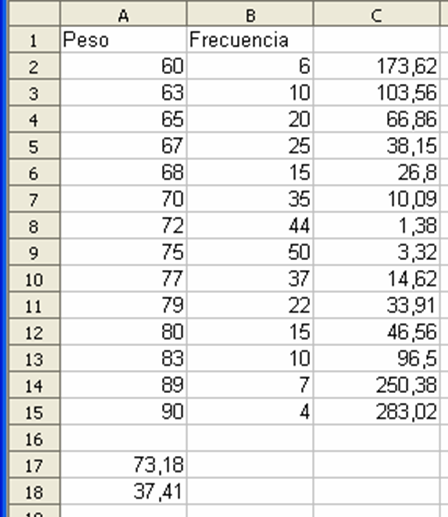
\includegraphics[width=7cm]{calc1ejem4T4.png}
\end{center}
\caption{Hoja de c\'alculo del ejemplo 3.}
\label{calc1ejem4T4}
\end{figure}

La varianza poblacional se habr\'ia calculado con la f\'ormula

\verb@=SUMA.PRODUCTO(B2:B15;C2:C15)/SUMA(B2:B15)@.

\end{enumerate}

\item La desviaci\'on t\'ipica se calcula como la ra\'iz cuadrada de la varianza:
nos colocamos por ejemplo en la casilla $A19$, escribimos la f\'ormula \verb@=RA�Z(A18)@
y pulsamos \textit{Enter}. El resultado es $6,12$.

\item El intervalo $[\bar{x}-2 s, \bar{x}+2s]$ es igual a: 
$[73,18-2 \cdot 6,12 \, , \, 73,18+2 \cdot 6,12]=[60,94, 85,42]$. Seg\'un la 
desigualdad de Chebichev en este intervalo debe haber un m\'inimo
de $1-\frac{1}{2^2}=0,75=75\%$ valores de la variable.
Podemos comprobar que, en efecto, esto es as\'i, ya que la frecuencias
de los valores en este intervalo suman: $10+20+25+15+35+44+50+37+22+15+10=283$.
Esto representa un $\frac{283}{300}=0,943=94,3 \%$ de los valores
de la variable.

\end{enumerate}



\vskip 0.5 cm
\noindent
\textbf{Ejemplo 4}

Calcular el rango intercuart\'ilico para la variable ``Edad de los condenados
en Baleares en 2005'' a partir de los datos de la siguiente tabla.
Suponiendo que la edad m\'axima es de 70 a\~nos, calcular el rango, la varianza y
la desviaci\'on est\'andar.

\begin{center}
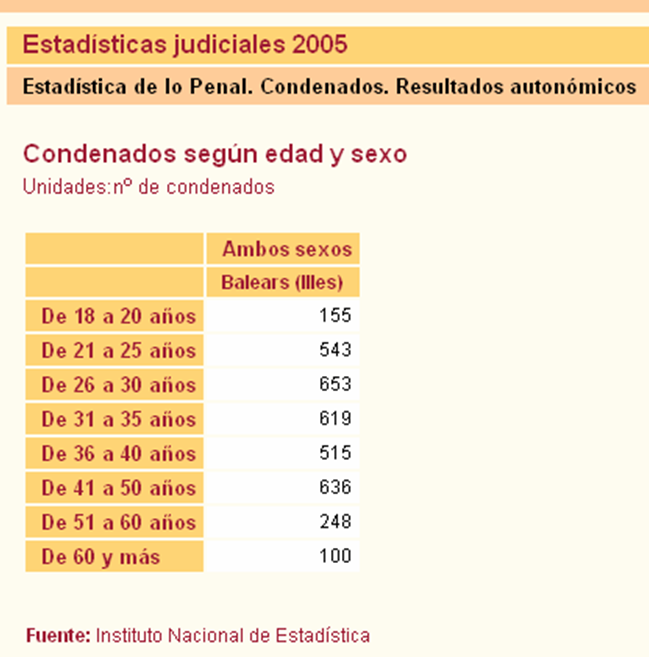
\includegraphics[width=12cm, height=8.5cm]{ejemplo3.png}
\end{center}

Los valores de media, mediana y cuartiles primero y tercero para este problema ya 
se calcularon en el ejemplo 4 del tema anterior:
\begin{center}
\begin{tabular}{ll}
Media (suponiendo edad m\'axima=70) & $35,43$ \\
Mediana & $33,48$ \\
$1^{er}$ cuartil & $27,04$ \\
$3^{er}$ cuartil & $42,65$ 
\end{tabular}
\end{center}

De aqu\'i deducimos que el rango intercuart\'ilico es $RIC=15,61$.
Por otra parte, el valor m\'inimo de la variable \textit{Edad} es $18$ y, seg\'un
el enunciado, el m\'aximo es $70$. De manera que el rango es $70-18=52$.

\vskip 0.2 cm
Para calcular la varianza debemos decidir primero qu\'e f\'ormula 
emplearemos (poblacional o muestral). En este caso, como disponemos 
de datos acerca de \emph{todos} los condenados en Baleares en 2005
consideramos que los datos se refieren a toda una poblaci\'on.
Procedemos del siguiente modo para hacer el c\'alculo:

\begin{enumerate}
\item Supongamos que el valor de la media (calculada en el ejemplo 4 del tema
anterior) se ha escrito en la casilla $A12$.
\item Creamos una nueva columna con los valores medios de cada intervalo,
tal como se ha explicado en el tema anterior.
\item Insertamos una nueva columna a la derecha de la columna $D$. Para ello situamos
el cursor sobre la parte superior de la columna $E$, hacemos clic en el bot\'on
derecho del rat\'on y elegimos la opci\'on \textit{insertar columnas}.
Una nueva columna $E$ aparece desplazando las que tiene a su derecha.
\item En la casilla $E2$ escribimos \verb@=(B2-$A$12)^2@.
Extendemos el c\'alculo al resto de casillas de la columna $E$ 
situando el cursor en la esquina inferior derecha 
de la casilla $E2$ y, manteniendo el bot\'on izquierdo del rat\'on pulsado, arrastrando
el cursor hasta la casilla $E9$. 
De esta manera en la columna E tenemos todos los factores $(x_i-\bar{x})^2$ de la
f\'ormula de la varianza. 
\item Finalmente, situamos en cursor en una casilla vac\'ia cualquiera, por ejemplo la casilla $A13$
y escribimos la f\'ormula 

\verb@=SUMA.PRODUCTO(B2:B9;E2:E9)/SUMA(B2:B9)@.

Al pulsar \textit{Enter} obtenemos el valor de la varianza poblacional en la casilla $A13$
(ver figura \ref{calc1ejem3T4}). El resultado final es $121,27$.

\begin{figure}[htbp]
\begin{center}
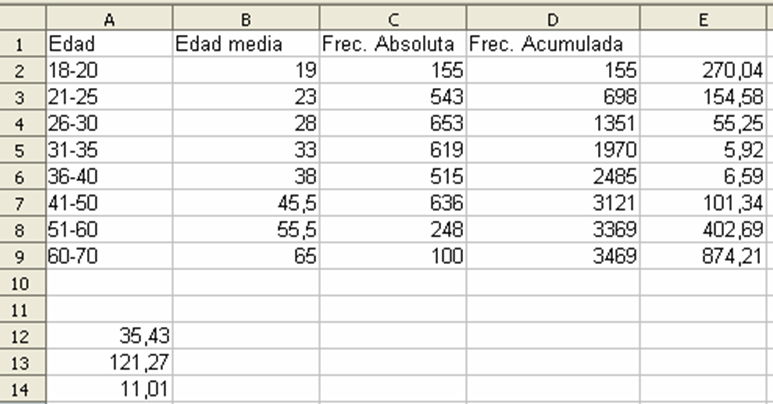
\includegraphics[width=12cm]{calc1ejem3T4.png}
\end{center}
\caption{Hoja de c\'alculo del ejemplo 4.}
\label{calc1ejem3T4}
\end{figure}

En caso de tener que calcular la varianza muestral hubi\'eramos utilizado la
siguiente f\'ormula: 

\verb@=SUMA.PRODUCTO(B2:B9;E2:E9)/(SUMA(B2:B9)-1)@.

\end{enumerate}


\vskip 0.2 cm
Finalmente calculamos la desviaci\'on t\'ipica como la ra\'iz cuadrada de la varianza:
nos colocamos por ejemplo en la casilla $A14$, escribimos la f\'ormula \verb@=RA�Z(A13)@
y pulsamos \textit{Enter}. El resultado es $11,01$.

\section{Ejercicios propuestos}

\vskip 0.2 cm
\noindent
\textbf{Ejercicio 1}

Calcular el rango, rango intercuart\'ilico, varianza, desviaci\'on est\'andar,
valores at\'ipicos y valores extremos para 
el n\'umero de farmacias por municipios en Mallorca
a partir de
los datos de la tabla \ref{ej1T4}.

\begin{table}[htbp]
\begin{center}
\caption{Farmacias en Mallorca, por municipio (fuente: Col.legi
Oficial d'Apotecaris de les Illes Balears, septiembre 2005)}
\label{ej1T4}
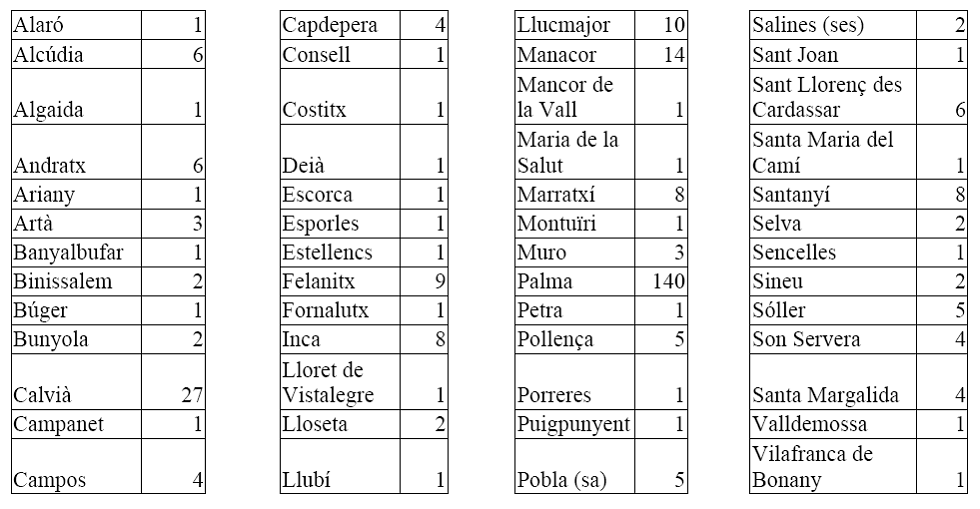
\includegraphics[width=14cm]{ej1T4.png}
\end{center}
\end{table}


\vskip 0.2 cm
\noindent
\textbf{Ejercicio 2}
 
A partir de los datos de la tabla \ref{ej2T4} calcular la media, la varianza y la desviaci\'on t\'ipica
de la variable ``Edad de v\'ictimas de accidentes en 2006''. 
\begin{table}[htbp]
\caption{Edad de v\'ictimas de accidentes en 2006 (fuente DGT)}
\label{ej2T4}
\begin{center}
\begin{tabular}{c|c}
Edad (a\~nos) & $N^o$ v\'ictimas \\ \hline
0 a 4 & 343 \\ 
5 a 14 & 1172 \\
15 a 17 & 333 \\
18 a 24 & 918 \\
25 a 64 & 5026 \\
65 a 80 & 2947
\end{tabular}
\end{center}
\end{table}


\vskip 0.2 cm
\noindent
\textbf{Ejercicio 3} 

Para incentivar a los trabajadores de una empresa de mensajeros 
la direcci�n de la empresa ha decidido conceder un suplemento salarial a la persona 
que hace las entregas con mayor rapidez. Los trabajadores de la empresa se organizan
en dos turnos. En el turno de la ma�ana, debido al tr�fico, el tiempo medio de entrega
es de $30$ minutos, con una varianza de $100$, mientras que en el turno de la
tarde la media es de $20$ minutos con una varianza de $49$. El mensajero m�s veloz
del turno de ma�ana tarda una media de $25$ minutos en hacer sus entregas y el de la tarde
$15$ minutos. Utiliza \textit{z-scores} para decidir a qu� mensajero aumentar el sueldo.


%\section{Soluciones de los ejercicios} 







